\begin{figure*}[!t]
\centering
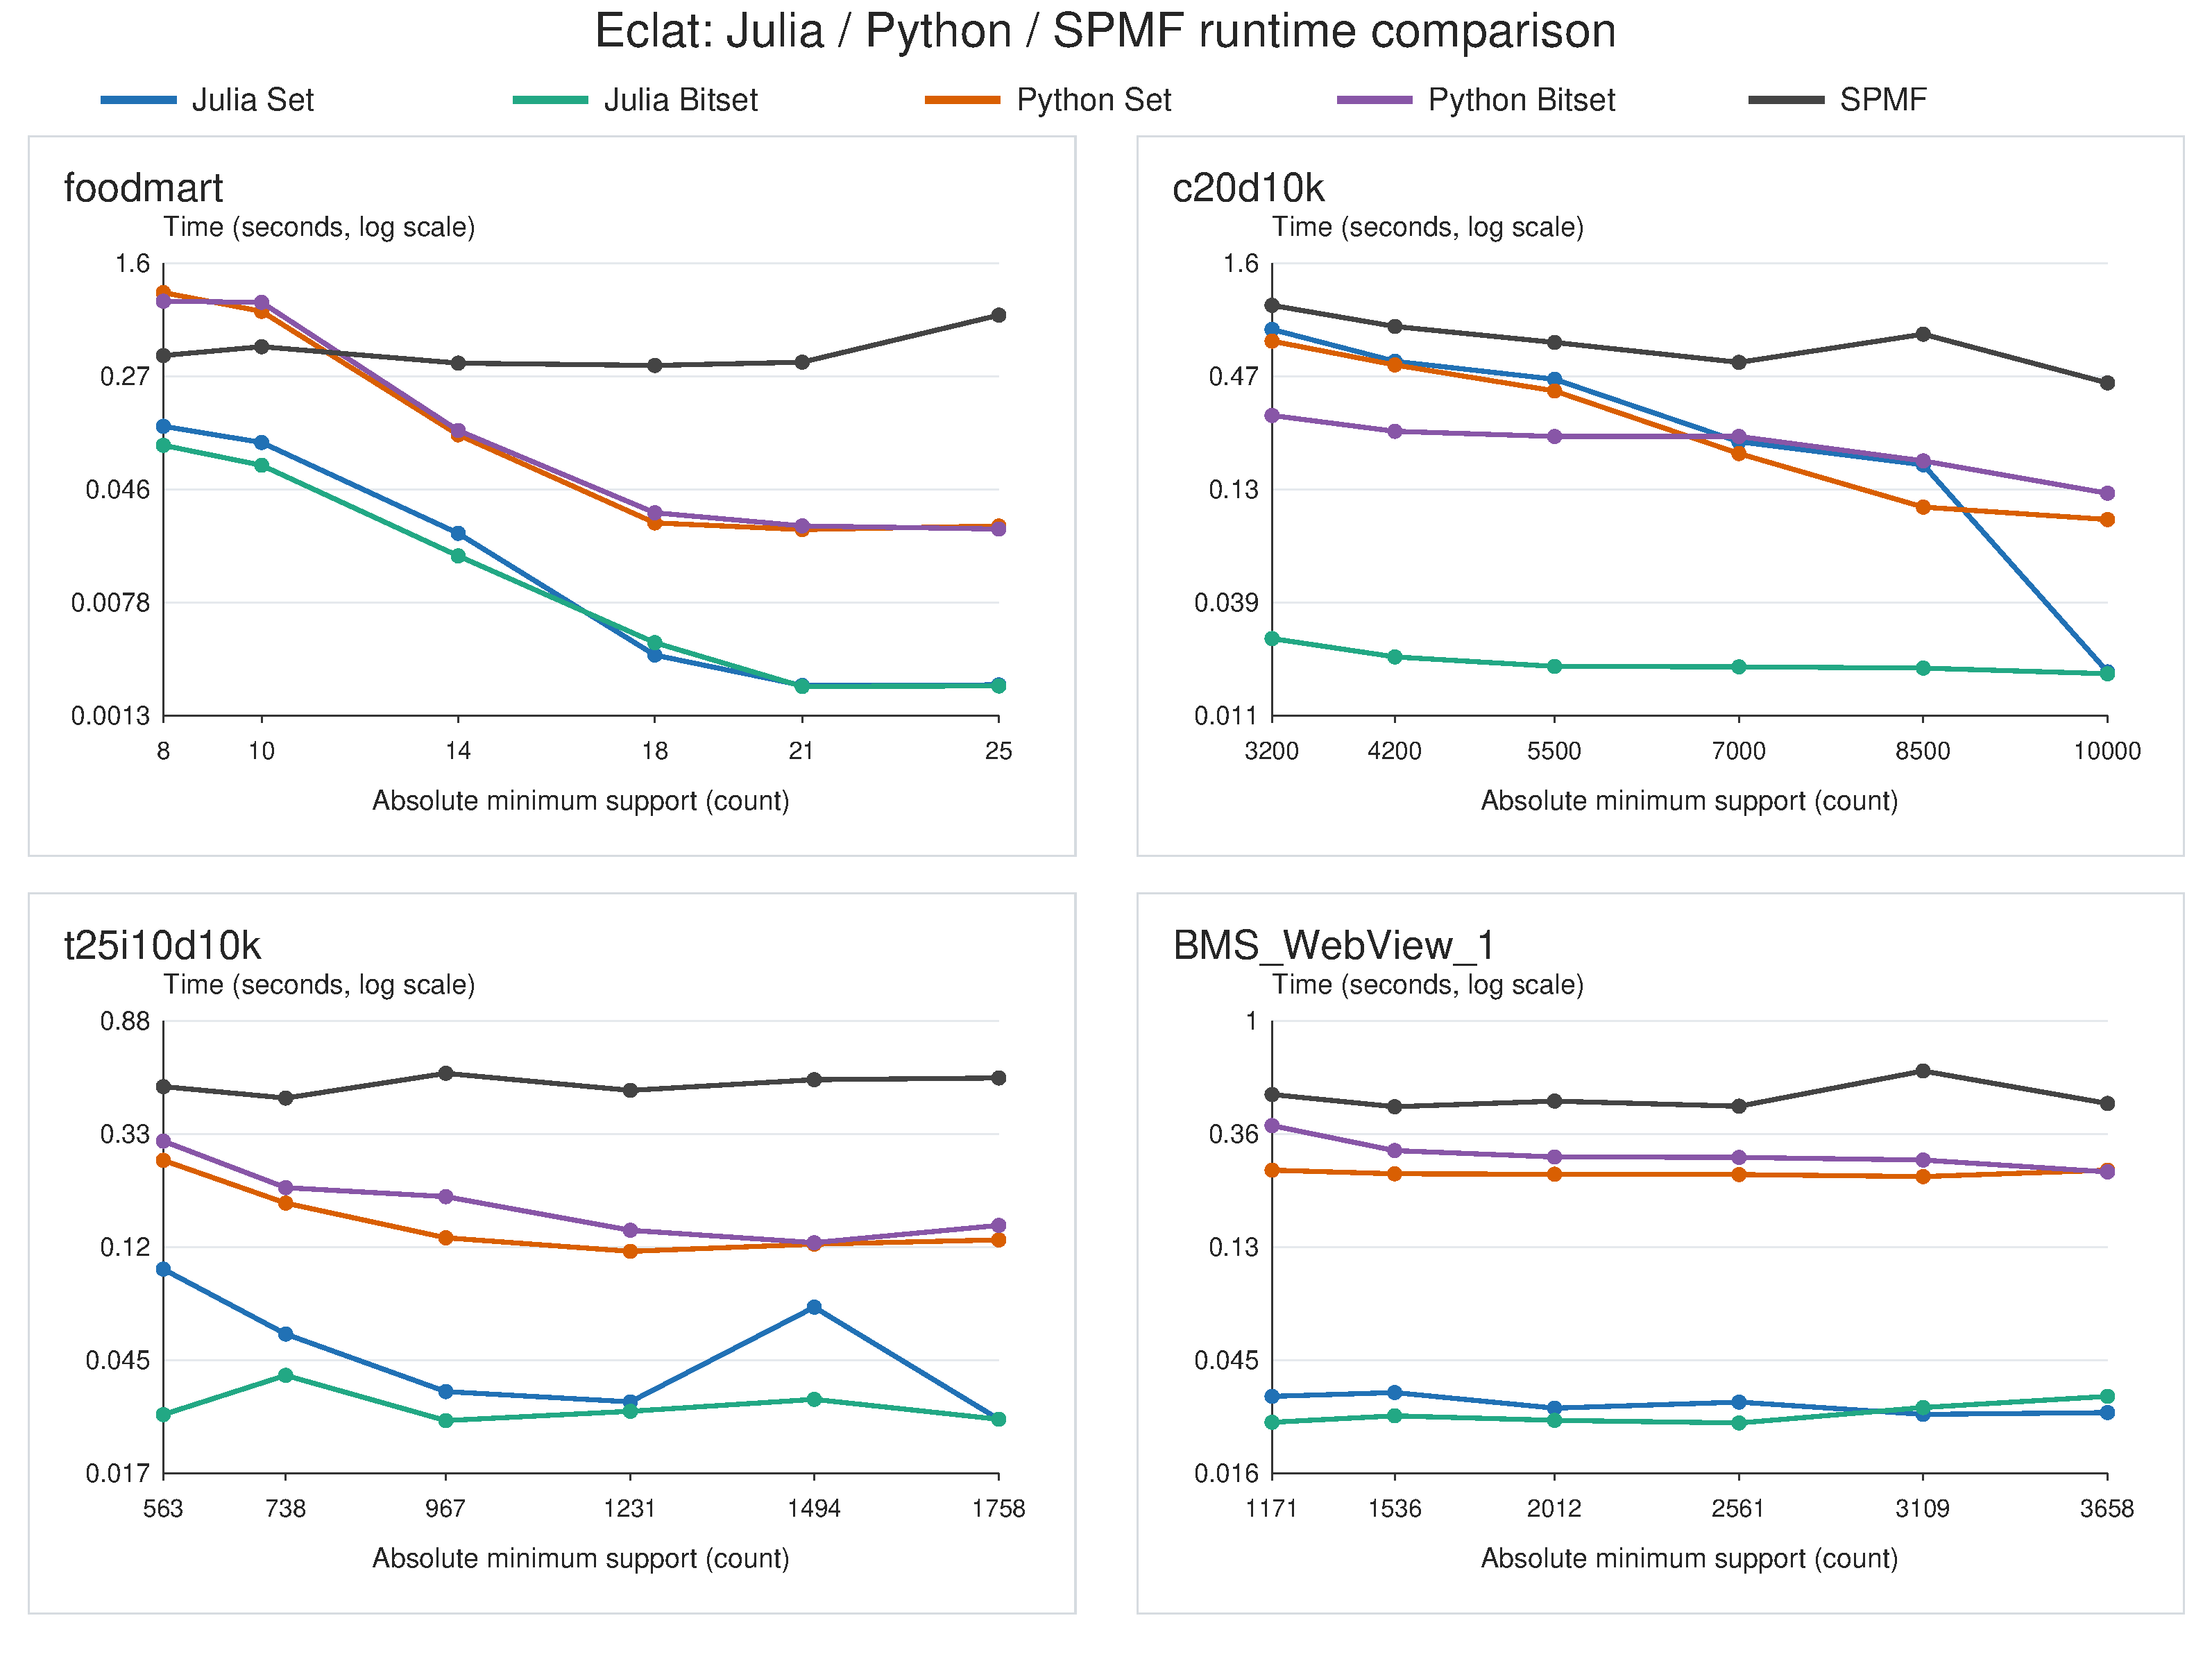
\includegraphics[width=\textwidth]{figures/julia_python_spmf_runtime.pdf}
\caption{Thời gian chạy Eclat trên bốn bộ dữ liệu với sáu mức minimum support: Julia (Set và BitVector), Python (set và bitset), và SPMF. Trục tung dùng thang logarit. Số liệu SPMF bao gồm khởi động JVM, trong khi thời gian Julia/Python được lấy từ benchmark riêng. Các phép đo không phải một so sánh hiệu năng thuần thuật toán trong điều kiện kiểm soát đồng nhất.}
\label{fig:julia-python-spmf-runtime}
\end{figure*}
Hình~\ref{fig:julia-python-spmf-runtime} tổng hợp kết quả thời gian của hai bản cài đặt do nhóm phát triển và SPMF. Mỗi mức support có một phép đo được ghi trong các tệp CSV của phiên chạy dùng để tạo đồ thị. Phần Julia và Python được thực hiện như các benchmark riêng, còn SPMF bao gồm chi phí khởi động JVM. Vì thế đồ thị mô tả số liệu quan sát, không đủ để kết luận tốc độ thuần thuật toán trên các môi trường thực thi khác nhau.
